In this chapter, an prototype of graphical discussion system will be created and make use of the previously developed approach as a "proof of concept". Firstly, ... the application domain will be presented and also foreshadow the prototype func- tionality. Afterwards, ... the development itself will take place, highlighting and documenting best practices in the subsequent sections.


\section{General}
On the whole, the implementation can be divided into two parts: client and server. Since they are fully separated, each part is considered and structured as a independent project. The implementation on client side is basically data fetching and template rendering, while data persistence and core business logic is implemented on the server side.  For convenience, the graphical discuss system is named \textbf{"Graphicuss"}, which stands for graphical plus discuss.


\subsection{Platform and Framework}
To achieve a better performance of view rendering on client side running in browser, React.js\footnote{https://facebook.github.io/react/ - accessed 10 July 2016} is taken as the front-end framework. Componentization, the main philosophy of ReactJS, also helps organize the views and view model logics. On the server side, ExpressJS\footnote{http://expressjs.com/ - accessed 12 July 2016} as a web framework is adopted for its efficiency and productivity of building RESTFul APIs.

Since both client and server projects are primarily implemented in JavaScript, NodeJS\footnote{https://nodejs.org/ - accessed 12 July 2016} is the single development environment for either project implementation or project management on both sides.

\subsubsection{File Structure}

To have a basic understanding of whole project including the server side and client side, a file structure of the project Graphicuss is listed in figure \ref{fig:overview-file-structure}:

\begin{itemize}
\item 
  \textbf{client/}: independent front-end project built on top of ReactJS
\item
  \textbf{server/}: independent back-end project implemented by using ExpressJS
\item
  \textbf{dist/}: compiled back-end project integrated with compiled and compressed static view files from front-end project
\item 
  \textbf{node\_modules/}: source of referenced third party libraries
\item 
  \textbf{package.json}: definition of third party libraries for client and server side
\item 
  \textbf{webpack.config.json}: config of specific behaviours in automated development or building process
\end{itemize}

\begin{figure}[!htbp]
\centering
\begin{forest}
  for tree={
    font=\ttfamily,
    grow'=0,
    child anchor=west,
    parent anchor=south,
    anchor=west,
    calign=first,
    edge path={
      \noexpand\path [draw, \forestoption{edge}]
      (!u.south west) +(7.5pt,0) |- node[fill,inner sep=1.25pt] {} (.child anchor)\forestoption{edge label};
    },
    before typesetting nodes={
      if n=1
        {insert before={[,phantom]}}
        {}
    },
    fit=band,
    before computing xy={l=15pt},
  }
[Graphicuss
  [client/]
  [server/]
  [dist/]
  [node\_modules/]
  [package.json]
  [webpack.config.js]
]
\end{forest}
\caption{Overview of Graphicuss' file structure}
\label{fig:overview-file-structure}
\end{figure}


\subsubsection{Module Management}

NodeJS provides native module management which is called \textit{npm}\footnote{https://www.npmjs.com - accessed 12 July 2016}. Third party libraries, which are published in the official remote repository, can be installed conveniently by only using npm's command line. There is also a list of names of all modules and dependencies in the file \textit{package.json}. Installing all dependencies and modules can be simply achieved by using only one command line \textit{npm install}, which will significantly ease the setting up process of the project freshly on a new machine.

\subsection{Architecture}

An architectural overview of Graphicuss is illustrated in figure \ref{fig:general-arch-imp}.

\begin{figure}[!htbp]
  \centering
    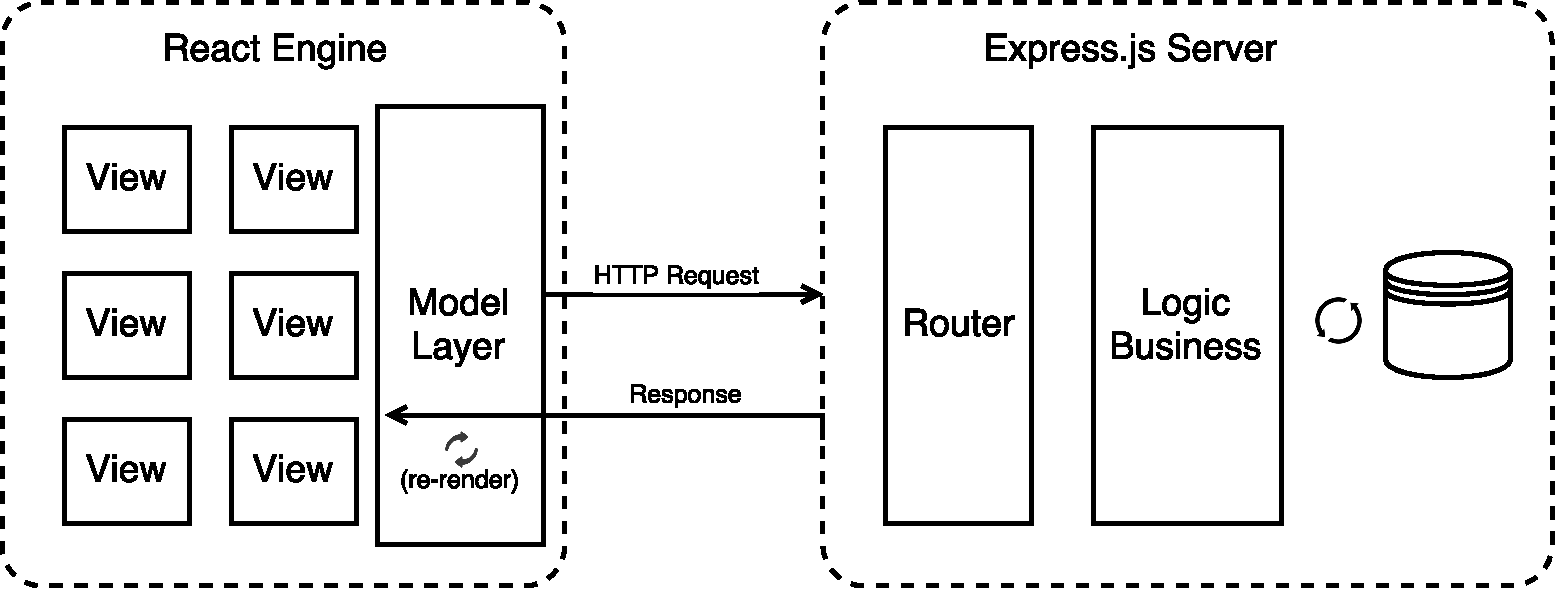
\includegraphics[width=1\textwidth]{Figures/imp-general-arch.pdf}
  \caption{General architecture}
  \label{fig:general-arch-imp}
\end{figure}
% Big Pic! Client with xuxian circle domain + React Engine -> Router in Express -> logic business + Database -> return 
While the client starts requesting a specific URL for data from the server, a HTTP connection will be established. The server program receives the HTTP request and forwards it to its router, in which rules for matching URLs have been pre-defined. By analysing headers of HTTP request, router will check if the request matches any pre-defined rules.

Not only the URL but also the parameters passed by client, for example the identifier of a resource, could also be extracted from HTTP headers. Server runs correlate business logics according to the rule of matched URL and executes operations of databases for data persistence. Afterwards, results are returned from server.

As soon as the data is successfully returned, the HTTP connection will be closed. The client processes data acquired from server, and represents it by re-rendering views. So far, a entire request over HTTP is accomplished.

\subsection{Automatization}
To accelerate the developing as well as building process of the project, a automatization tool called \textit{Webpack}\footnote{https://webpack.github.io/ - accessed 13 July 2016} is used. 

Webpack is a tool which could analyse the dependencies of the project and bundle modules with the app. In addition, it can also do tasks like compressing JavaScript codes to reduce the size of the client app, or compiling modern JavaScript as well as CSS codes to achieve the compatibility for old browsers.

\subsubsection{Automated Development Process}
To make the development of client app independent, it will start a dev server on its own for development purpose. However the dev server started by client app and the actual server are running on different ports. Which means that the communication between them will cause CORS problem.

CORS means, a resource makes a cross-origin HTTP request when it requests a resource from a different domain than the one which the first resource itself serves. For security reasons, browsers restrict cross-origin HTTP requests initiated from within scripts. \cite{CORS}

Through configuring the dev server started by Webpack, a proxy could established to forward request to the actual back-end server. As figure \ref{fig:proxy-server-imp} shows, the client is able now to request APIs under the same domain, and requests will go though the dev server, after that they are forwarded to the actual server.

\begin{figure}[!htbp]
  \centering
    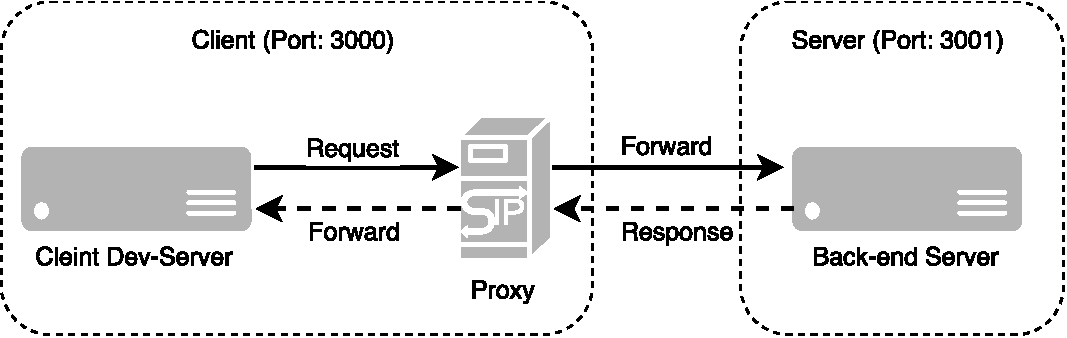
\includegraphics[width=1\textwidth]{Figures/imp-proxy-server.pdf}
  \caption{Proxy for client development server}
  \label{fig:proxy-server-imp}
\end{figure}
% Dev Process, in development(dev server, proxy) + building)


\subsubsection{Automated Building Process}

For the client app, multiple tasks are executed during the building process by using Webpack: transforming modern JavaScript code, pre-processing the modern CSS code and bundling the static files. All these tasks will significantly reduce the size of client app and also improve the compatibility of the app.

Webpack also helps accelerate the building process by defining various automated building tasks. It will bundle all dependencies with the server app and client app. After processing on both sides, the final output of the files will be extracted into the \textit{dist} directory mentioned in \ref{fig:overview-file-structure}, which is now ready for deploying and serving. The whole building process is represented in figure \ref{fig:automated-building-imp}.

\begin{figure}[!htbp]
  \centering
    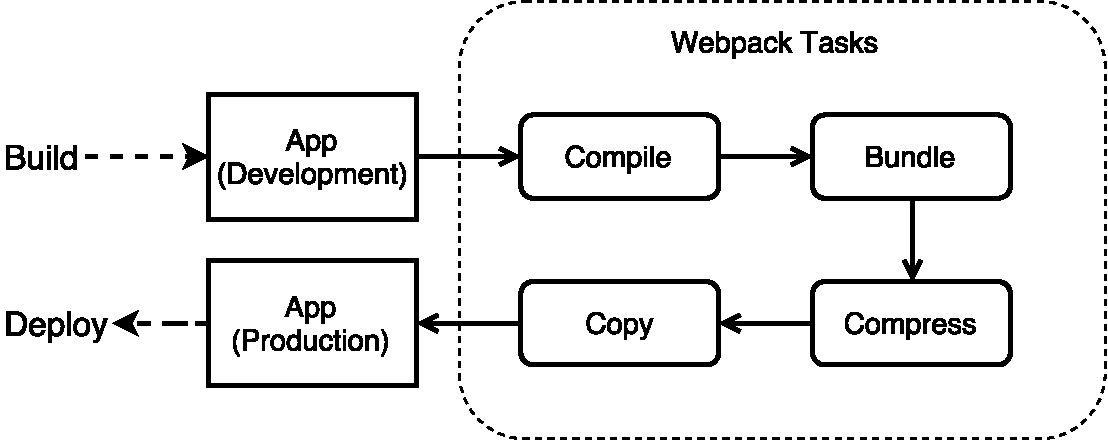
\includegraphics[width=1\textwidth]{Figures/imp-automated-building.pdf}
  \caption{Automated building process with Webpack}
  \label{fig:automated-building-imp}
\end{figure}
% Building Process, a->b->c->d xuxian kuang, Webpack compile, bundle, compress -> copy file to dist -> ready for deploy

\subsection{Storage Structure} \label{subsec:storage-structure-imp}
In section \ref{sec:data-concept}, data domains and fields of data domains  have already been defined. 

For all persistence storage of data on the server side a MongoDB\footnote{https://www.mongodb.com/ - accessed 13 July 2016} database is used.  In figure \ref{fig:data-model-table-imp}, more concrete definition of data model table is defined. MongoDB is a non-SQL database, which uses document oriented storage and JSON style data model. That will make it easy to implement as well as scale data models. In addition, An \gls{ORM} framework called Mongoose\footnote{http://mongoosejs.com/ - accessed 13 July 2016} is also applied to the implementation, which encapsulates the native database operations of MongoDB. With help of the \gls{ORM} framework, definition of schema and query on database will be quite simple. 

% Description othe the table?

\begin{figure}[!htbp]
  \centering
    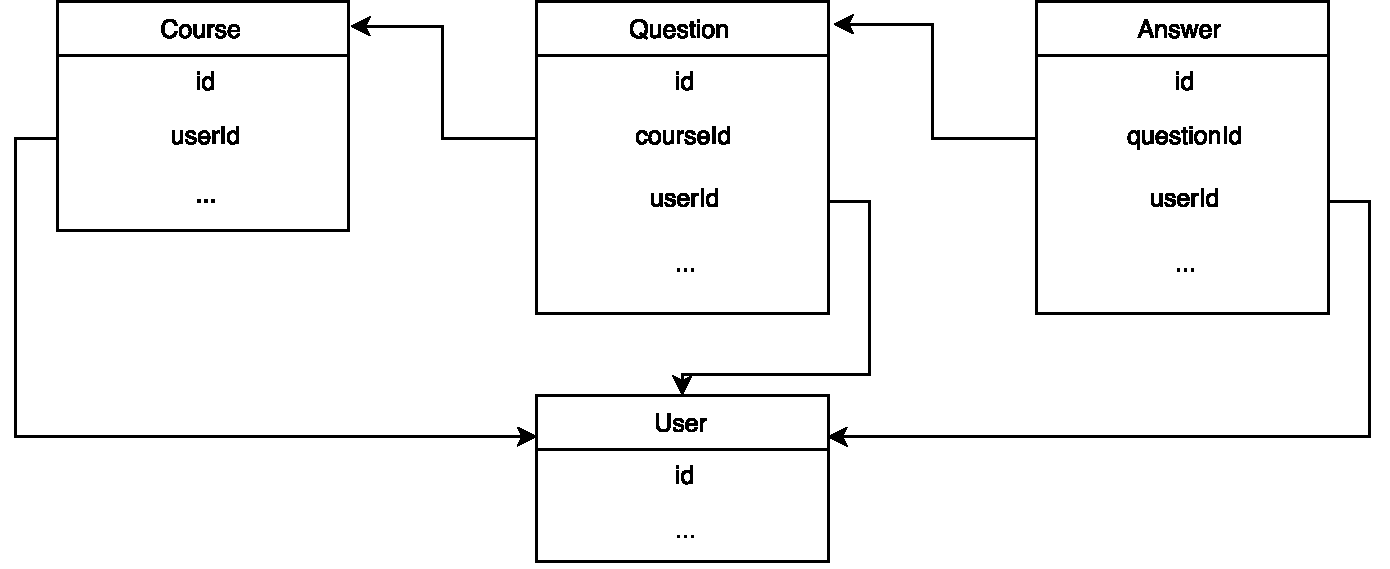
\includegraphics[width=1\textwidth]{Figures/concept-data-domain-relation.pdf}
  \caption{Table of data model}
  \label{fig:data-model-table-imp}
\end{figure}
% Whole Concret Data Model Table

 % File Structure, Data Design, Workflow(automated)

\section{Server of Graphicuss}
This section gives the explanation of architectural pattern and more detailed implementation of the server side. 

% Architecture MV, , JWT for Auth, Websocket Dispatcher, Resource Listening?

\subsection{Architecture}

\subsubsection{MVC Pattern and Project Structure}
To separate the different layers of model, view and controller, \gls{MVC} pattern is used as the basic pattern of the architecture. In the model layer, all data model related concerns such as data shema definitions, data model validation as well as database operations are defined. And Controllers contain the core domain logics, process the data from model layer, and pass the result to view layer.

Since the templates are rendered on the client side, the view layer is just simply stripped. Therefore, basically the controllers response processed data to client side directly without rendering it to views. Figure \ref{fig:server-file-structure-imp} shows the overview of the server's  file structure which is featured with MVC pattern.

\begin{figure}[!htbp]
\centering
\begin{forest}
  for tree={
    font=\ttfamily,
    grow'=0,
    child anchor=west,
    parent anchor=south,
    anchor=west,
    calign=first,
    edge path={
      \noexpand\path [draw, \forestoption{edge}]
      (!u.south west) +(7.5pt,0) |- node[fill,inner sep=1.25pt] {} (.child anchor)\forestoption{edge label};
    },
    before typesetting nodes={
      if n=1
        {insert before={[,phantom]}}
        {}
    },
    fit=band,
    before computing xy={l=15pt},
  }
[server
  [config/
    [index.js]
    [routes.js]
  ]
  [models/]
  [controllers/]
  [index.js]
  [...]
]
\end{forest}
\caption{Overview of server app's file structure}
\label{fig:server-file-structure-imp}
\end{figure}


\begin{enumerate}
\item 
  \textbf{index.js}: the entry point of the whole server app. It will create a server instance and set up configurations for the server. In addition, a connection from server instance to database will be established. After all configurations are done, the server instance will start listening port and waiting for the requests from client.
\item
  \textbf{config/index.js}: config as well as constants for the server. It persists \textit{apiConfig} for example the common prefix of API URL and version of the API. And config for database including the database URL will be defined here as well. In addition, keys for encryption are also stored in the config file.
\item
  \textbf{config/routes.js}: rules for URL matching. All URL matching rules are defined in this file. Controllers are referenced here and a dispatcher for router will be instantiated. If any request meets the defined rule, the request will be forward to a correlative controller. 
\item
  \textbf{controllers/*}: controllers for processing specific requests.
\item 
  \textbf{models/*}: data model definitions. Files under this directory are organized by different data domain.
\end{enumerate}


\subsubsection{Achitecture of Server}

The figure \ref{fig:server-arch-imp} illustrates an overview of the server's architecture. 

\begin{figure}[!htbp]
  \centering
    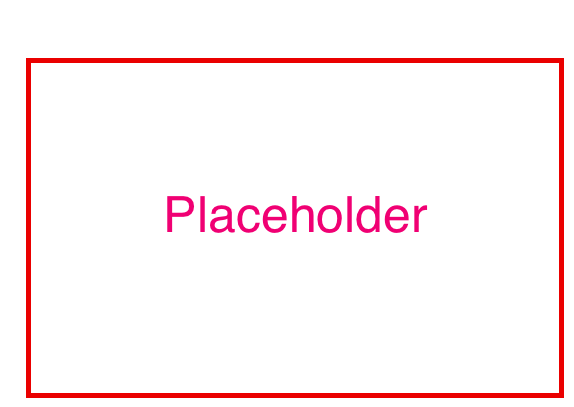
\includegraphics[width=0.6\textwidth]{Figures/placeholder.png}
  \caption{placeholder}
  \label{fig:server-arch-imp}
\end{figure}
% process of request to be handeled. index.js -> create server isntance -> connect to database. routes -> different controllers -> different models

\subsection{Data Schema Definition}
% Architecture MV, , JWT for Auth, Websocket Dispatcher, Resource Listening?

\section{Client of Graphicuss}



\subsection{Architecture}
For the implementation of the client application, \textit{React.js} which aims to solve the challenges involved when developing web application with complex user interfaces, is applied. To have a better concept of how Graphicuss's client application is implemented, an overview of the file structure is listed in the figure \ref{fig:client-file-structure-imp}.

\subsubsection{Project Structure}
\begin{figure}[!htbp]
\centering
\begin{forest}
  for tree={
    font=\ttfamily,
    grow'=0,
    child anchor=west,
    parent anchor=south,
    anchor=west,
    calign=first,
    edge path={
      \noexpand\path [draw, \forestoption{edge}]
      (!u.south west) +(7.5pt,0) |- node[fill,inner sep=1.25pt] {} (.child anchor)\forestoption{edge label};
    },
    before typesetting nodes={
      if n=1
        {insert before={[,phantom]}}
        {}
    },
    fit=band,
    before computing xy={l=15pt},
  }
[client
  [components/
    [AppBar/
      [index.js]
      [style.css]
    ]
    [...]
  ]
  [containers/]
  [models/]
  [utils/]
  [index.js]
  [index.html]
  [...]
]
\end{forest}
\caption{Overview of client app's file structure}
\label{fig:client-file-structure-imp}
\end{figure}

\begin{itemize}
  \item 
  \textbf{components/}: all components are defined by extending basic \textit{React.Compoent}. Each custom component has an \textit{index.js}, which processes the logics of view rendering and applies view model to the template. \textit{style.css} defines the CSS style of the HTML DOMs within a component.
  \item 
  \textbf{containers/}: containers are compositions of components.
  \item 
  \textbf{models/}: in model directory, data models for the components are defined. In addition, the definition of APIs and processing after data acquisition  also take place here.
  \item 
  \textbf{index.js \& index.html}: \textit{index.js} is the entry point of the app, which will instantiate the React instance and render the views into a specific DOM defined  in \textit{index.html}
\end{itemize}


\subsubsection{Achitecture of Client}

An overview of the client application's architecture is revealed in figure \ref{fig:client-arch-imp}. 

\begin{figure}[!htbp]
  \centering
    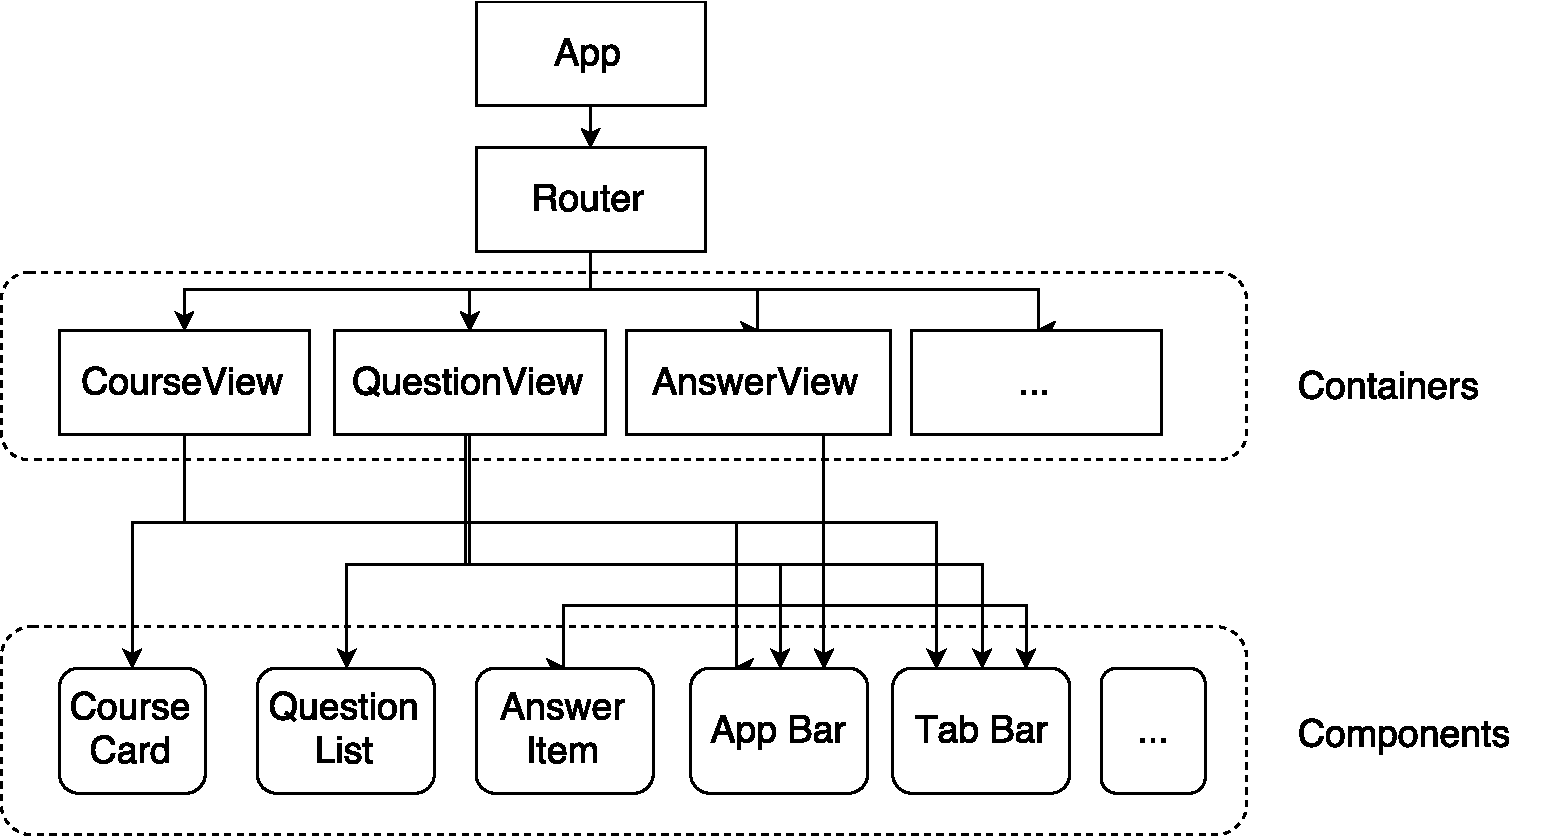
\includegraphics[width=1\textwidth]{Figures/imp-client-arch.pdf}
  \caption{Overview of client architecture}
  \label{fig:client-arch-imp}
\end{figure}
% client arch, App -> router containes rotes -> different container -> components(Compisition... for containers!) xuxian for layer (App, router, container, components)

In the React application, \textit{Router} is also regarded  as a component, in which different matching rules of URL are defined. If the URL requested by user is matched, a correlate view will be rendered according to the definition of routes. Code list \ref{list:router-client-imp} shows the implementation of defining a \textit{Router} component.

\begin{lstlisting}[language=HTML, caption=Router in client app , label={list:router-client-imp}]
<Router history={history}>
  <Route path="/" component={App}>
    <Route path="auth" component={AuthView} />
    <Route path="courses" component={CoursesView} />
    <Route path="courses/:courseId" component={QuestionsView} />
    <Route path="questions/:questionId" component={AnswersView} />
  </Route>
</Router>
\end{lstlisting}

Containers such like \textit{CourseView}, \textit{QuestionsView} or \textit{AnswersView} are compositions of components in fact. The way how component acquires view model is that the parent component pass values to its child component by defining the properties of the child component. So the data flow starts from the root component and goes through every child components. 

How to manage the data flow and control the rendering behaviour will be discussed later in the sub section \ref{subsection:data-flow-react-imp}.


\subsection{Composition of Components}

\subsubsection{React Component}

Defining a new \textit{Component} with React.js must extent the \textit{React.Component} class and implement the \textit{render()} function, which will be called when the component is instantiated. Afterwards, the template as well as the composition of components are rendered to plain HTML.  A simplfied example of building a \textit{CourseView} component is represented in code list \ref{list:course-view-render-imp}.

\begin{lstlisting}[language=HTML, caption=Rendering \textit{CourseView} with multiple \textit{CourseCard} components , label={list:course-view-render-imp}]
class CoursesView extends React.Component {
  render() {
    const courses = this.props.courses
    return (
      <div>
        {
          courses.map( (course) =>
            <CourseCard course={course} key={course._id}></CourseCard>
          )
        }
      </div>
    ); 
  }
}
\end{lstlisting}

As mentioned above, the parent components pass data through as the properties of child components. Within the \textit{CoursesView}, \textit{courses} could be read from its properties which is defined while \textit{CourseView} is composed. In the \textit{render()} function of \textit{CourseView}, \textit{courses} are traversed and each single \textit{course} will be passed into the \textit{CourseCard} as its property. Which means, as \textit{CourseView} is rendered, all \textit{CourseCard} components within it will also call their own \textit{render()} functions with the data model passed in. Data flows from top to bottom, likewise, views are rendered from parent to children components.

\subsubsection{Composition}
\textit{Components} are the core of React. All each view and its view model of the client application is represented as a React \text{Component}. And the whole client app is actually a composition of React components. An example of \textit{CoursesView} is taken in figure \ref{fig:course-view-composition-imp}.

\begin{figure}[!htbp]
  \centering
    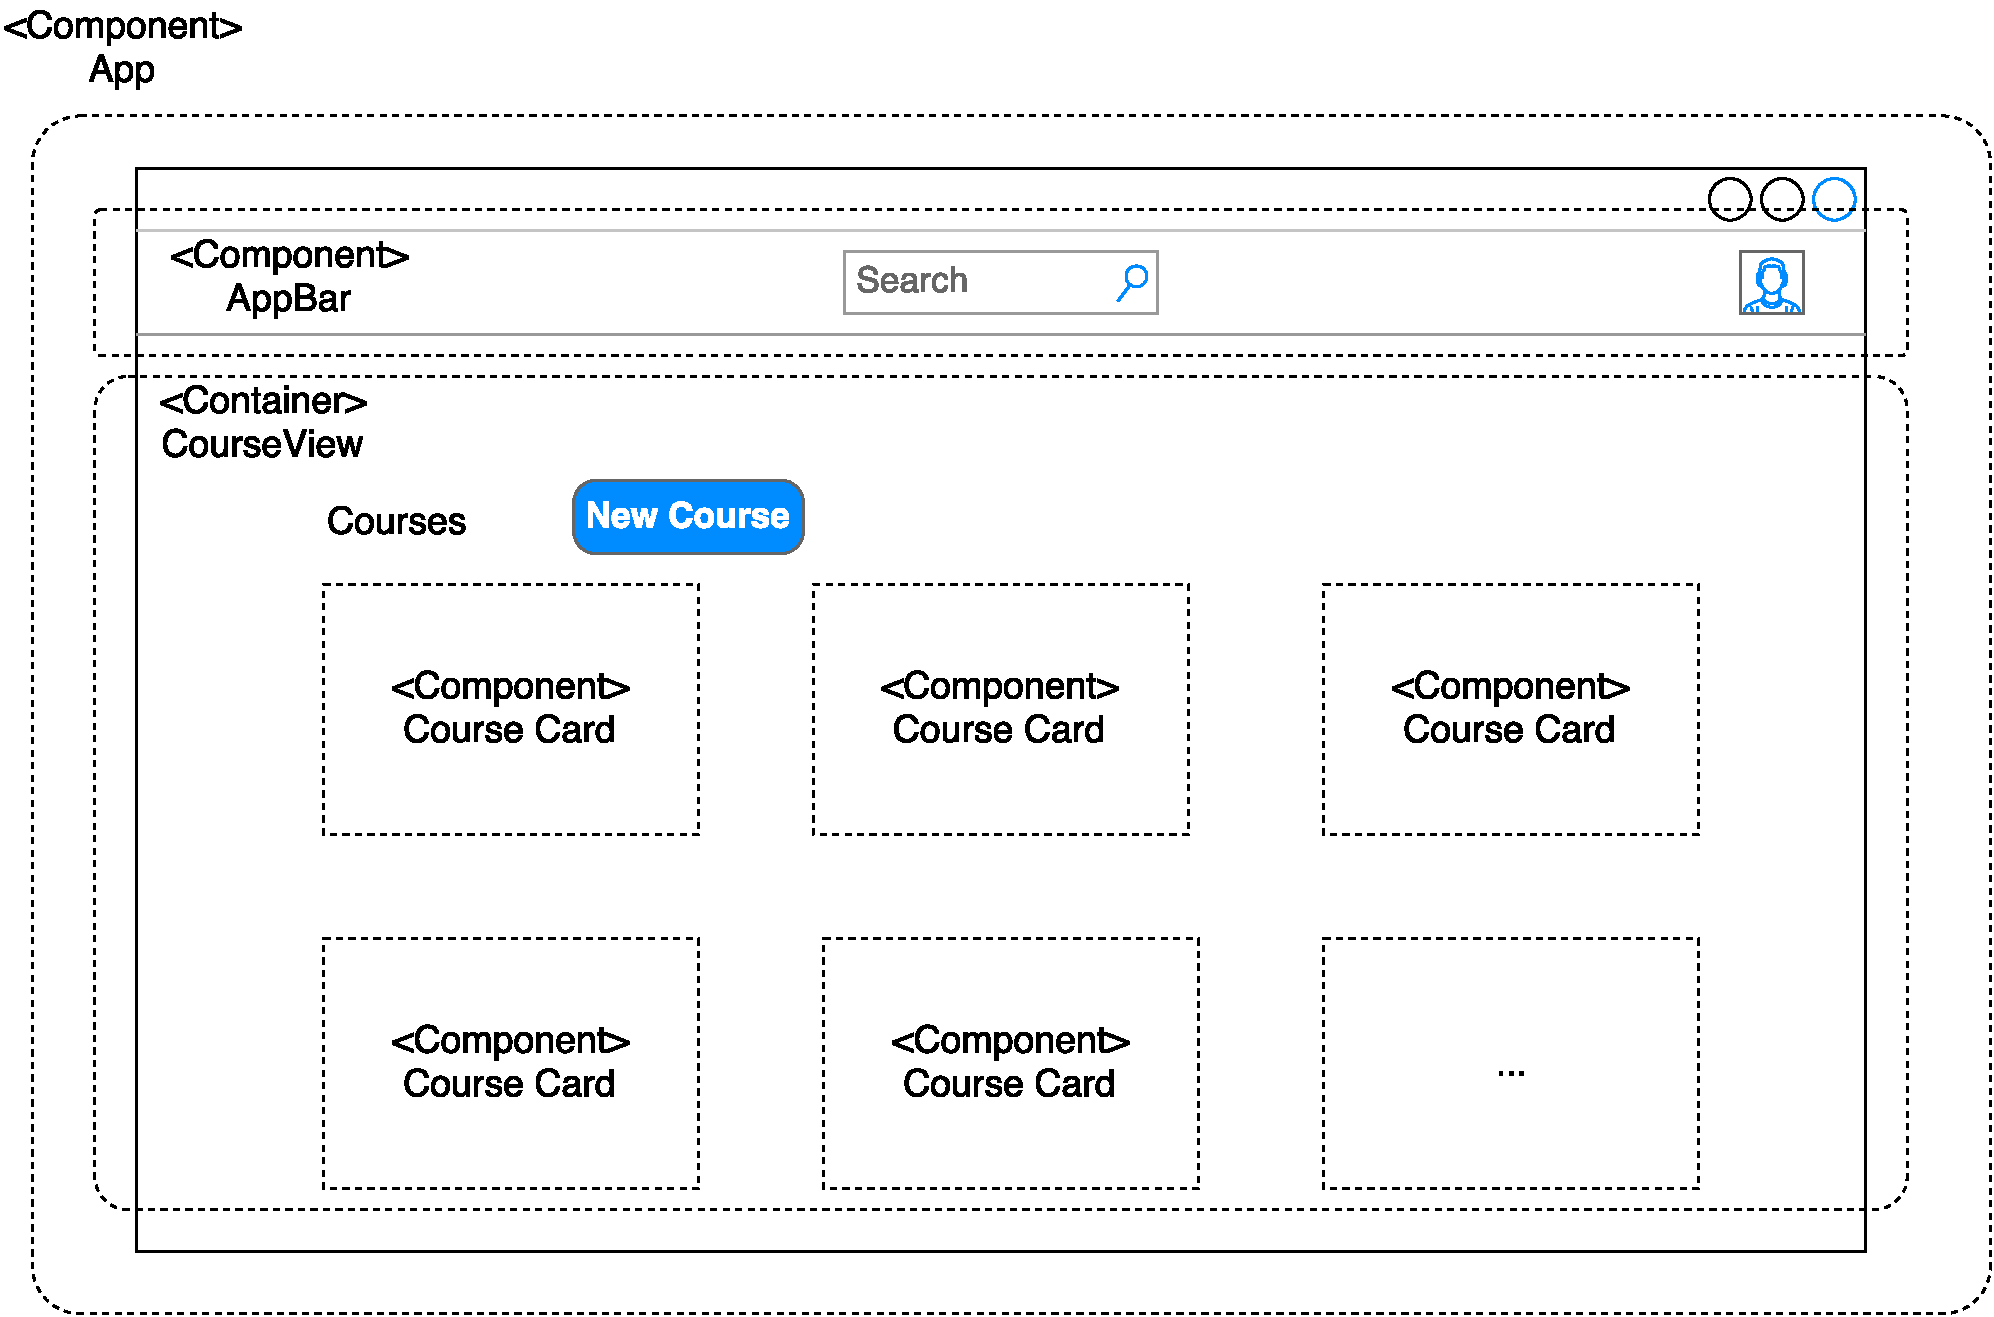
\includegraphics[width=1\textwidth]{Figures/imp-course-view-composition.pdf}
  \caption{Composition of components in courses' page}
  \label{fig:course-view-composition-imp}
\end{figure}
% Course Page. Composition, App bar, tab view, course page, course card ...

At the top of the view is a component called \textit{AppBar}, which is also composed with another component \textit{SearchBox}. \textit{ContentSection} is a container for the main content, which will be replaced and re-rendered if the context of router changes. In this example, the route \textit{/courses} is applied, and the component \textit{CourseView} is rendered into \textit{ContentSection}. 

\textit{CourseView} is also a composition of components: a list of \textit{CourseCard} components and also other components such as submit button component and popover component for creating new course. 

In principle, building other views is the same approach. Composition of components constructs the all views. With fine-grained components, the client app becomes much extensible and maintainable.


\subsection{Data Flow}\label{subsection:data-flow-react-imp}

Since data is passed as properties of components from top to bottom in the React application, maintaining data models between components and the data flow through components is a problem. \textit{Flux}\footnote{http://facebook.github.io/flux/} is a architecture which aims to solve this problem. Data flows in single direction, which keeps the process simple and ensures the correctness of view rendering.

There are four main concepts of Flux architecture: 
\begin{itemize}
  \item 
  \textbf{View}: view layer which references the data model and renders the data model into template.
  \item 
  \textbf{Action}: action made by view, trigger for processing data model, for example a mouse click event.
  \item 
  \textbf{Dispatcher}: receives the actions and run callback functions to modify the data model.
  \item 
  \textbf{Store}: stores the states of data, if the states of data are changed, store will notify the views to re-render with the new state of data.
\end{itemize}

\begin{figure}[!htbp]
  \centering
    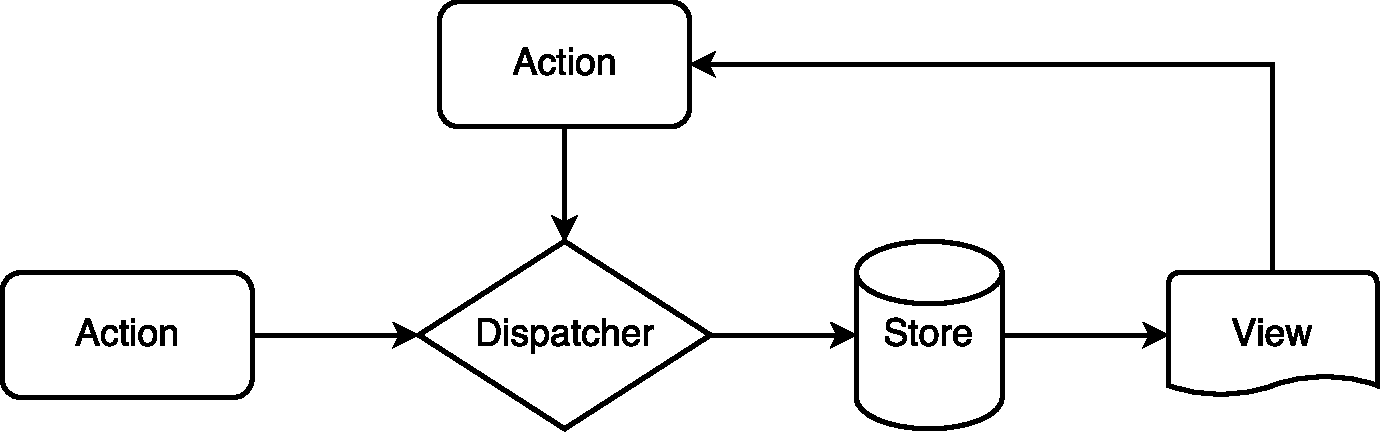
\includegraphics[width=0.9\textwidth]{Figures/imp-flux-arch.pdf}
  \caption{Data flow in Flux architecture}
  \label{fig:flux-arch-imp}
\end{figure}

The main process of data flow in Flux architecture is illustrated in figure \ref{fig:flux-arch-imp}. The key of Flux is unidirectional data flow. For example, user wants to submit a new answer to a certain question in Graphicuss system, as soon as the new answer is synchronized with server side, the new answer will be rendered into the answer list attached to the question. The process of data flow in this case is described as following:
\begin{enumerate}
  \item 
  User submits a new answer, \textit{Action(NEW\_ANSWER)} is triggered.
  \item 
  \textit{Action} requests the API for submitting new answer.
  \item 
  \textit{Dispatcher} receives the \textit{Action(NEW\_ANSWER)} and inserts an entry of this new answer into the \textit{answers} state which is stored in \textit{Store}.
  \item 
  Since the state of \textit{answers} is changed, \textit{Store} starts notifying the views to re-render.
  \item 
  Views re-render the templates with the new state of \textit{answers} which contains the new submission of answer.
\end{enumerate}
% Architecture Building Tool, Compile Workflow, Whiteboard, Socket, React?

\section{Drawing Tool for Graphicuss}
In this section, the implementation of converting Canvas to a storable data with JSON format is introduced. Afterwards, a drawing tool which provides user interfaces to draw various elements on Canvas is implemented.

\subsection{Objectified Canvas}

\subsubsection{Fabric.js}
Fabric.js\footnote{http://fabricjs.com/ - accessed 18 July 2016} is a powerful and simple Javascript HTML5 canvas library, which provides interactive object models on top of canvas elements. Since native Canvas only provides low-level APIs for creating elements, but not maintains the life cycle of elements on itself. Fabric.js solves this problem with objectifying native elements and encapsulating native methods for drawing elements. 

Instead of dealing with low-level APIs natively provided by Canvas, Fabric.js provides objectified model for elements with different shapes  on top of native methods. It takes charge of canvas state and rendering, make it possible to manipulate objects directly.


\subsubsection{Serialized Canvas}
Since all elements on the Canvas drawn by Fabric.js can be maintained as an object with properties like position, size and styles.
So the Canvas within Fabric.js can be simply serialized to a JSON object or other formats. 

Fabric.js provides a helper function called \textit{toJSON()}, which will serialize the canvas with canvas properties as well as all object models on the canvas. Code list \ref{list:serialized-canvas-imp} is an example that shows how the serialized output looks like if a rectangle object is created by using Fabric.js.

\begin{lstlisting}[language=JavaScript, caption=Serialized Canvas by Fabric.js , label={list:serialized-canvas-imp}]
var canvas = new fabric.Canvas();
canvas.backgroundColor = 'red';
canvas.add(new fabric.Rect({
  left: 50,
  top: 50,
  height: 20,
  width: 20,
  fill: 'green'
}));
console.log(JSON.stringify(canvas));
/* --- Output of serialized Canvas --- 
{"objects":[{"type":"rect","left":50,"top":50,"width":20,"height":20,"fill":"green","overlayFill":null,"stroke":null,"strokeWidth":1,"strokeDashArray":null,"scaleX":1,"scaleY":1,"angle":0,"flipX":false,"flipY":false,"opacity":1,"selectable":true,"hasControls":true,"hasBorders":true,"hasRotatingPoint":false,"transparentCorners":true,"perPixelTargetFind":false,"rx":0,"ry":0}],"background":"rgba(0, 0, 0, 0)"}
*/
\end{lstlisting}

Comparing with output generated by native Canvas mentioned in section \ref{sec:graphical-data-serialization-concept}, this serialized JSON object is not only efficient for storing, but also has the possibility for restoring all object models and re-rendering them on Canvas.

\subsection{Drawing Tool}
The drawing tool is developed on top of the library Fabric.js. It provides the functionalities such as drawing, styling, dragging and resizing of various elements. Not only graphical elements, texts could also be rendered and styled on the Canvas while using drawing tool.

Figure \ref{fig:drawing-tool-arch-imp} illustrates an overview of the drawing tool's architecture. 

\begin{figure}[!htbp]
  \centering
    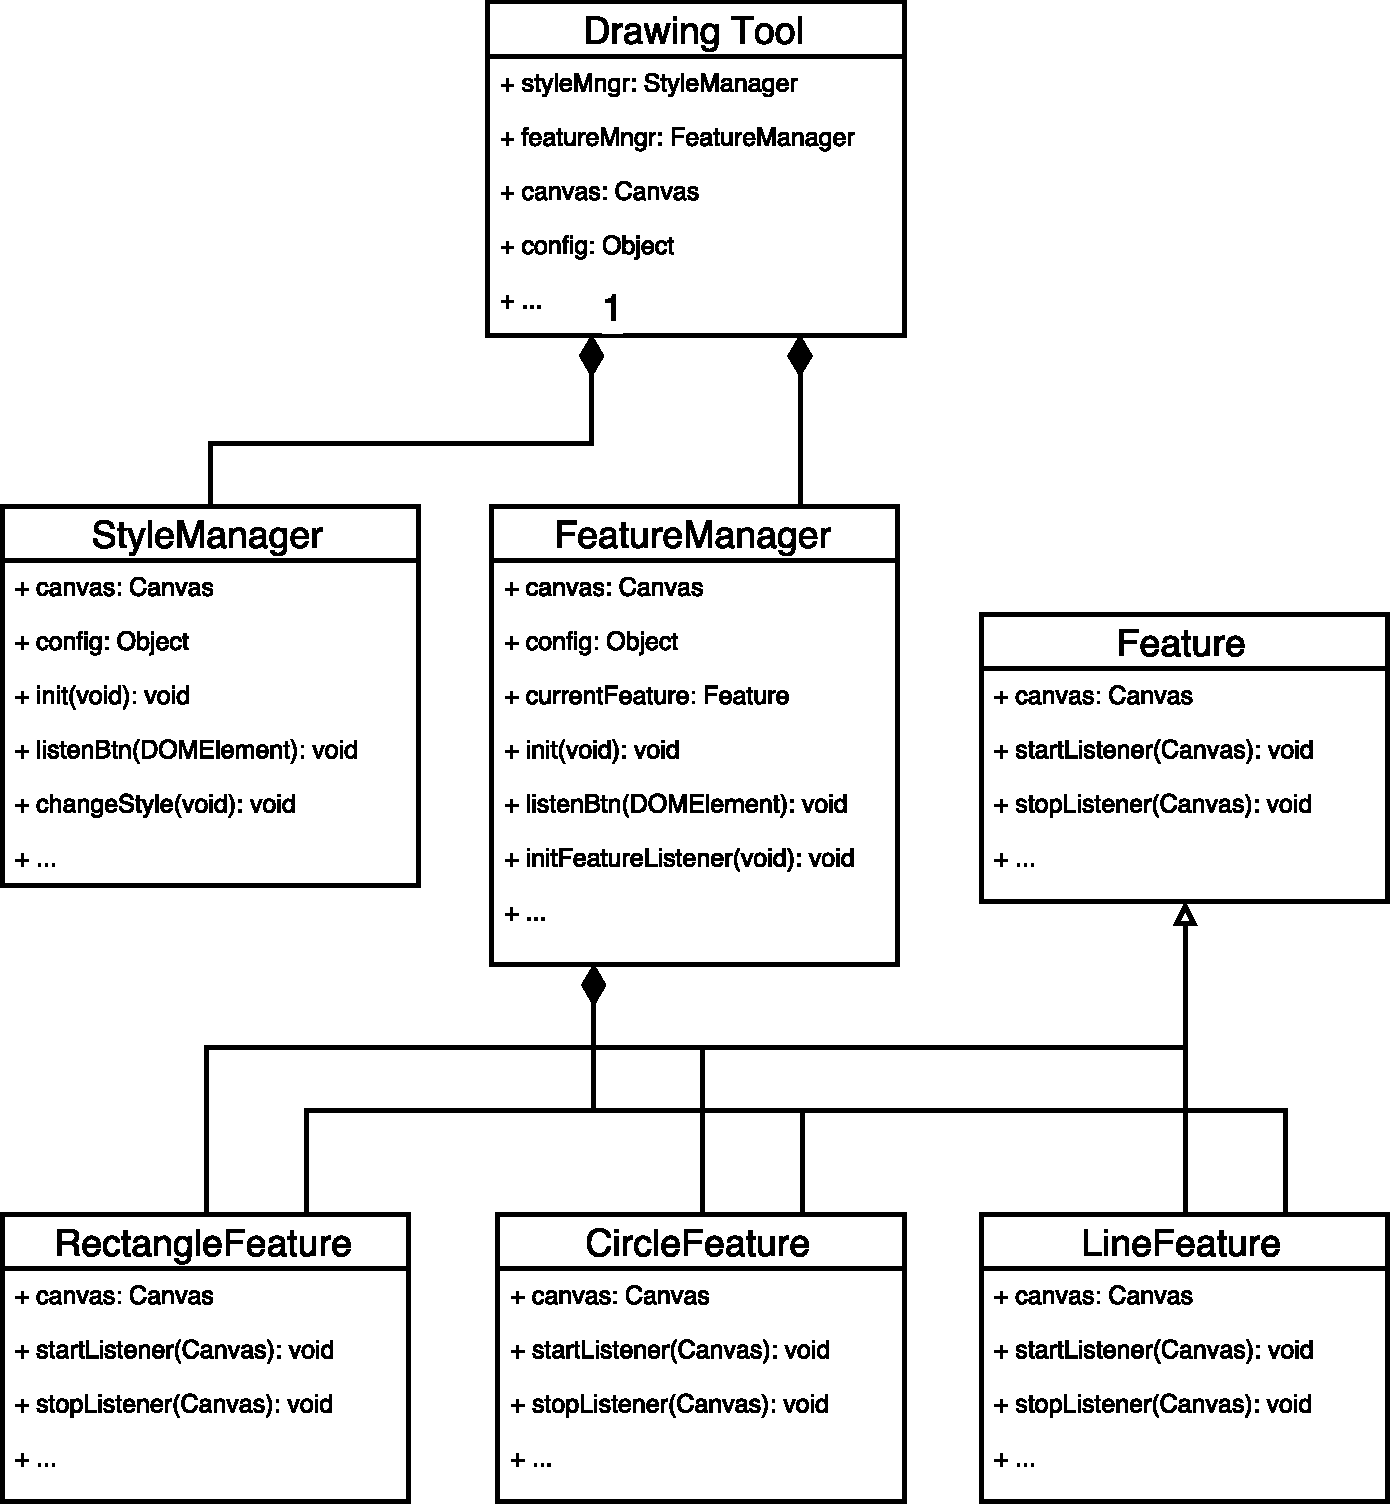
\includegraphics[width=1\textwidth]{Figures/imp-drawing-tool-arch.pdf}
  \caption{Architecture of drawing tool}
  \label{fig:drawing-tool-arch-imp}
\end{figure}

\subsubsection{Style Manager}
At the startup of drawing tool, \textit{StyleManager} is instantiated. \textit{StyleManager} receives the config instance, in which the DOM elements with relevant styling functionalities are defined. And in the \textit{init()} function of \textit{StyleManager}, listeners for the DOM elements are created. If the DOM elements are triggered by the user, \textit{StyleManager} will apply the chosen style to the active objects on the Canvas.

Code list \ref{list:style-manager-imp} takes the listener for DOM element of color picker, which is used for changing the color of an object on Canvas. It acquires the reference of color picker DOM from the config instance, and starts listening for the \textit{onchange} event. If the \textit{onchange} event is fired, the listener will set the object's \textit{fill} property to the color value. Afterwards, the canvas is re-rendered and the active object with new color is shown up.

\begin{lstlisting}[language=JavaScript, caption=Main process of StyleManager, label={list:style-manager-imp}]
class StyleManager {
  constructor(canvas, config){
    this._canvas = canvas;
    this._config = config;
  }
  init(){
    el = this._config['color-picker-dom']
    this._listenColor(el)
    // ... more styling listeners
  }
  _listenColor(el){
    let self = this;
    el.onchange = function(){
      var obj = self.canvas.getActiveObject();
      self._setObjStyle(obj, 'fill', el.value);
      canvas.renderAll();
    }
  }
  // ...
}
\end{lstlisting}


\subsubsection{Feature Manager \& Extensible Features}

In addition, a \textit{FeatureManager} is also created for managing different drawing functionalities. The basic idea of \textit{FeatureManager} is quite similar as \textit{StyleManager} mentioned above. It also listens for the DOM elements to toggle different drawing behaviours.

After that a specific drawing mode is triggered by user, \textit{FeatureManager} will assign listeners for specific mouse events on the Canvas and track the drawing behaviours. According to the mouse events triggered by user on the Canvas, the correlate objects will be rendered into the Canvas context.

\begin{lstlisting}[language=JavaScript, caption=Main process of FeatureManager, label={list:feature-manager-imp}]
class FeatureManager {
  constructor(canvas, config){
    this._canvas = canvas;
    this._config = config;
  }
  init(){
    el = this._config['text-feature-dom']
    this._listenText(el)
    // ... more features' listeners
  }
  _listenText(el){
    let textFeature = new TextFeature(this._canvas);
    el.onclick = (e) => { 
      this._clickHandler(text)
    }
  }
  // ...
}
class TextFeature{
  constructor(canvas){
    this._canvas = canvas;
  }
  startListen(){
    // tracking mouse event
  }
  stopListen(){
    // remove listeners
  }
}
\end{lstlisting}

Features, namely drawing modes are highly extensible on the drawing tool. \textit{TextFeature} in code list \ref{list:feature-manager-imp} is an example. All feature classes need to implement two interfaces \textit{startListen()} and \textit{stopListen()} basically. In \textit{startListen()}, listeners for tracking mouse events are defined. And in \textit{stopListen()}, all listeners should be removed. Both functions will be called by \textit{FeatureManager} when this drawing mode is toggled.

\section{Difficulties and open Questions}
% increment history!


\section{Conclusion}
Conclusion!
